\documentclass[19pt,landscape]{article}
\usepackage[landscape]{geometry}
\geometry{a5paper,scale=0.8}
\usepackage{listings}
%\geometry{left=1.5cm,right=1.5cm,top=1.5cm,bottom=0.5cm}
\usepackage{booktabs}
\usepackage{color}
% \usepackage{ulem} % for strikethrough
\usepackage{amsfonts}
\usepackage{Sweave}
\usepackage{bm}
\usepackage{graphicx} 
\usepackage{amsfonts,amsmath,latexsym,amssymb,mathrsfs,amsthm,mathtools}
\usepackage{xr} % [cross-referencing] 
\externaldocument[L3-]{Lecture3} % [cross-referencing] 
% \usepackage[british]{babel}
%\usepackage[T1]{fontenc}
%\usepackage{mathptmx}
% \usepackage{times}
\usepackage{datetime2}
\usepackage{filemod}
% \usepackage{fontspec}    %change font 
% \setmainfont{Times New Roman}%fontspec下这个命令设置全局默认字体
\newtheorem{thm}{Theorem}%[section]
\newtheorem{prop}[thm]{Proposition}
\newtheorem{defi}[thm]{Definition}
\newtheorem{lma}[thm]{Lemma}
\newtheorem{cor}[thm]{Corollary}
\newtheorem{exam}[thm]{Example}
\newtheorem{countexam}[thm]{Counterexample}
\newtheorem{rem}[thm]{Remark}
\newtheorem{con}[thm]{Conjecture}
%\bracketfactory{floor}{\lfloor}{\rfloor}
\usepackage{enumerate}
\usepackage{color}
%\usetheme{Copenhagen}
\usepackage[english]{babel}
\usepackage[utf8x]{inputenc}
\newcommand{\law}{\mathscr{L}}
\newcommand{\HH}{\mathscr{H}}
\newcommand{\D}{\mathbb{D}}
\newcommand{\IP}{\mathbb{P}} 
\newcommand{\bone}{{\bf 1}}
\DeclareMathOperator{\E}{\mathbb{E}}
\DeclareMathOperator*{\esssup}{ess\,sup}
\newcommand{\IE}{\E}
\newcommand{\mean}{\E}
\newcommand{\R}{\mathbb{R}}
\newcommand{\N}{\mathbb{N}}
\newcommand{\non}{\nonumber}
\newcommand{\Z}{\mathbb{Z}}
\newcommand{\C}{\mathbb{C}}
%\newcommand{\C}{{\mathds{C}}}
\newcommand{\ci}{{\cal I}}
\newcommand{\cf}{{\cal F}}
\newcommand{\LL}{\textbf{L}}
\DeclareMathOperator{\Var}{\mathrm{Var}}
\DeclareMathOperator{\var}{\mathrm{Var}}
\DeclareMathOperator{\cov}{\mathrm{Cov}}
\DeclareMathOperator{\corr}{\mathrm{Corr}}
\DeclareMathOperator{\bs}{\mathrm{Bias}}
\DeclareMathOperator{\bigo}{\mathrm{O}}
\newcommand{\K}{\textbf{Ker}}
\newcommand{\Id}{\textbf{Id}}
\newcommand{\Pn}{{\rm Pn}}
\newcommand{\dtv}{{d_{\rm TV}}}
\newcommand{\dk}{{d_{\rm K}}}
\newcommand{\dw}{{d_{\rm W}}}
\def\tg{{\tilde g}}
\def\a{{\alpha}}
\def\cn{{\mathcal{N}}}
\def\equald{\stackrel{\mbox{\scriptsize{{\rm d}}}}{=}}
\def\ER{Erd\H{o}s-R\'enyi}
\usepackage{color} 
\definecolor{lightblue}{rgb}{0,0.2,0.5}
\usepackage[colorlinks=true, urlcolor=lightblue,linkcolor=lightblue, citecolor=lightblue]{hyperref}

%%%%%%%%%%%%%%%%%%%%%%%%%%%%%%%%%%

%%% Define bracket commands
\def\given{\mskip 0.5mu plus 0.25mu\vert\mskip 0.5mu plus 0.15mu}
\newcounter{@bracketlevel}
\def\@bracketfactory#1#2#3#4#5#6{
\expandafter\def\csname#1\endcsname##1{%
\addtocounter{@bracketlevel}{1}%
\global\expandafter\let\csname @middummy\alph{@bracketlevel}\endcsname\given%
\global\def\given{\mskip#5\csname#4\endcsname\vert\mskip#6}\csname#4l\endcsname#2##1\csname#4r\endcsname#3%
\global\expandafter\let\expandafter\given\csname @middummy\alph{@bracketlevel}\endcsname
\addtocounter{@bracketlevel}{-1}}%
}
\def\bracketfactory#1#2#3{%
\@bracketfactory{#1}{#2}{#3}{relax}{0.5mu plus 0.25mu}{0.5mu plus 0.15mu}
\@bracketfactory{b#1}{#2}{#3}{big}{1mu plus 0.25mu minus 0.25mu}{0.6mu plus 0.15mu minus 0.15mu}
\@bracketfactory{bb#1}{#2}{#3}{Big}{2.4mu plus 0.8mu minus 0.8mu}{1.8mu plus 0.6mu minus 0.6mu}
\@bracketfactory{bbb#1}{#2}{#3}{bigg}{3.2mu plus 1mu minus 1mu}{2.4mu plus 0.75mu minus 0.75mu}
\@bracketfactory{bbbb#1}{#2}{#3}{Bigg}{4mu plus 1mu minus 1mu}{3mu plus 0.75mu minus 0.75mu}
}


% \title{Nonparametric Regression}
% \author{Qingwei Liu}
% \institute{National University of Singapore}
% \date{\today}

\begin{document}
% \maketitle
%
\setkeys{Gin}{width=0.16\textwidth}
% \begin{titlepage}
% \begin{center}
%     \vfill
% \textbf{\huge ST5207 Nonparametric Regression\\
% Semester 1, AY2024/25}\\[4cm]
% \begin{minipage}{0.4\textwidth}
% \begin{center} \large
% Lecturer:~Qingwei Liu\\
% % Email:liu\_qw@nus.edu.sg\\
% \vskip 6pt
% Department of Statistics and Data Science\\
% \vskip 6pt
% National University of Singapore
% \end{center}
% \end{minipage}%\\[1cm]
% \vfill
% % \includegraphics[width=0.1\textwidth]{./logo}\\[0.5cm]
% \vfill
% \end{center}

% \end{titlepage}
%

\newpage
{\LARGE\centerline{\textbf{Lecture~4:~Bandwidth Selection Methods}\footnote{Last modified in \filemodprintdate{Lecture4}.}}}
\vskip25pt
\begin{minipage}{.9\textwidth}
    \Large
\begin{itemize}
\item Reference Method
\begin{itemize}
    \item Silverman's Rule of Thumb
\end{itemize}
\item Plug-in Method
    \item Cross-Validation 
    \begin{itemize}
        \item Maximum Likelihood Cross-Validation
        \item Least-Squares Cross-Validation
    \end{itemize}

\end{itemize}
More details can be found in \cite{hall91minima}, \cite{hall91lower}, \cite{hall92smoothed}, \cite{hardle12}.
\end{minipage}

\newpage
{\Large\centerline{\textbf{Motivation}}}
\vskip25pt
\begin{minipage}{.9\textwidth}
    \Large
    The choice of bandwidth $h$ is the main problem of kernel density estimation. 
    
    Why? The bandwidth $h$ of the kernel estimator controls the smoothness of the resulting curve estimate.

    An ideal solution of selecting the bandwidth should be both applicable in practice, and theoretically desirable as well. 

    Recall the global optimal bandwidth, Eq.~\eqref{L3-optbin1} in Lecture 3,
    \begin{equation*}
        h^*=\left[\frac{\|K\|_{L^2}^2}{\var(Z)^2\|f''\|_{L^2}^2}\right]^{1/5}n^{-1/5}. 
    \end{equation*}
One thing need to keep in mind: the kernel $K$ is known, and the density $f$ is not.
\end{minipage}



\newpage
{\LARGE\centerline{\textbf{Rule-of-Thumb Bandwidth}}}
\vskip25pt
\begin{minipage}{.9\textwidth}
    \Large 
   We try to estimate $\|f''\|^2_{L^2}$, assuming $f$ to belong to a pre-specified family of density functions. For example, we assume the unknown distribution be $\mathcal{N}(\mu,\sigma^2)$. Then we have 
   \begin{eqnarray*}
    \|f''\|^2_{L^2}&=&\sigma^{-5}\int_{\R}\phi''(x)^2\mathrm{d}x\\
    &=&\frac38 \pi^{-1/2}\sigma^{-5}\approx0.212\sigma^{-5},
   \end{eqnarray*}
   where $\phi(x)=\frac1{\sqrt{2\pi}}e^{-x^2/2}$ is the p.d.f. of standard normal distribution. 
If a Gaussian kernel is being used, then the bandwidth is 
\begin{eqnarray}
    \hat{h}_{rot}&=&\left[\frac{\|\phi\|_{L^2}^2}{\frac38 \pi^{-1/2}\sigma^{-5}}\right]^{1/5}n^{-1/5}\nonumber\\
    &=&(3/4)^{1/5}\sigma n^{-1/5}\approx1.06\sigma n^{-1/5}
\end{eqnarray}
    \end{minipage}

    \newpage
    {\LARGE\centerline{\textbf{Kernel Density Estimators}}}
    \vskip25pt
    \begin{minipage}{.9\textwidth}
        \Large 
       The {\it kernel density estimator} may be written compactly as 
       \begin{equation}\label{def-kde}
        \hat{f}(x):=\frac1{nh}\sum_{i=1}^nK\left(\frac{x-X_i}h\right)=\frac1n\sum_{i=1}^nK_h(x-X_i),
       \end{equation}
        where $K_h(t):=K(t/h)/h$. 
        \vskip5pt
        \begin{itemize}
            \item The function $K(\cdot)$ is referred as {\it kernel function}, e.g. those given in Table~\ref{tabkernels}, and $h$ denotes the bandwidth.
            \item $K_h$ is the {\it bandwidth-rescaled kernel function.}
            \item In practice, kernel functions $K(\cdot)$ are chose to be (symmetric) probability density functions, i.e. $\int K(x)\mathrm{d}x=1$ and $K(x)\ge0$ for all $x\in\R$.
            \item If $K(\cdot)$ is a prob. density function, so is $K_h(\cdot)$, for any $h>0$.
        \end{itemize}
        \end{minipage}

\newpage
{\LARGE\centerline{\textbf{Kernel functions}}}
\vskip25pt
\begin{table}[h!]
    \centering
    \renewcommand{\arraystretch}{2} % Adjust the row height
    \begin{tabular}{|c|c|c|}
        \hline
        \textbf{Kernel} & \textbf{Formula} & \textbf{Properties} \\
        \hline
        Uniform & \( K(u) = \frac{1}{2} \mathbf{1}(|u| \leq 1) \) & Simple, piecewise constant \\
        \hline
        Triangular & \( K(u) = (1 - |u|) \mathbf{1}(|u| \leq 1) \) & Continuous, piecewise linear \\
        \hline
        Epanechnikov & \( K(u) = \frac{3}{4} (1 - u^2) \mathbf{1}(|u| \leq 1) \) & Optimal MISE \\
        \hline
        Quartic (Biweight) & \( K(u) = \frac{15}{16} (1 - u^2)^2 \mathbf{1}(|u| \leq 1) \) & Smoother, reduces boundary effects \\
        \hline
        Triweight & \( K(u) = \frac{35}{32} (1 - u^2)^3 \mathbf{1}(|u| \leq 1) \) & Very smooth \\
        \hline
        Gaussian & \( K(u) = \frac{1}{\sqrt{2\pi}} \exp\left(-\frac{u^2}{2}\right) \) & Infinite support, very smooth \\
        \hline
        Cosine & \( K(u) = \frac{\pi}{4} \cos\left(\frac{\pi u}{2}\right) \mathbf{1}(|u| \leq 1) \) & Smooth and continuous \\
        \hline
    \end{tabular}
    \caption{Commonly Used Kernels in Nonparametric Regression}
    \label{tabkernels}
\end{table}

\newpage
{\LARGE{\textbf{Examples of Kernels}}}
\vskip25pt
   
%\begin{figure}[h]
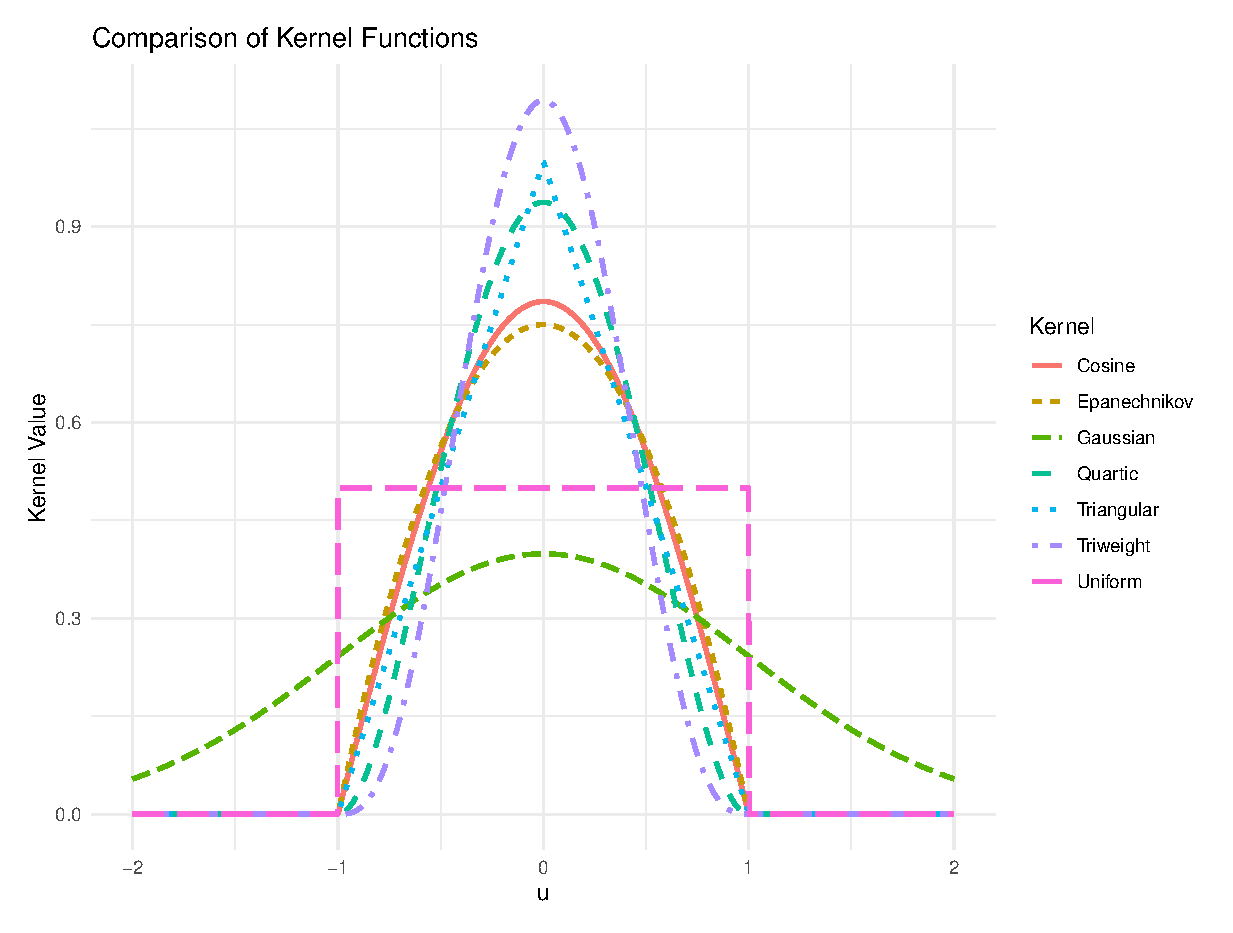
\includegraphics[width=0.9\textwidth,height=0.5\textwidth]{kernel_comparison.eps}
%\end{figure}

\newpage
{\LARGE\centerline{\textbf{Convolutions}\footnote{\cite[Chapter V, Section~4]{fellerv2}.} }}
\vskip25pt
\begin{minipage}{0.9\textwidth}
    \Large 
    Let $\phi$ be a bounded function, $F$ be a probability distribution with density function $f$. The convolution of a function $\phi$ with a probability function $F$ is given by 
    \begin{equation}
        \left(f*\phi\right)(x):=\int_{\R}\phi(x-y)F\{\mathrm{d}y\}=\int_{\R}\phi(x-y)f(y)\mathrm{d}y.
    \end{equation}
    {\bf Claim~1:} If $\phi$ is bounded and continuous, so is $f*\phi$. If $\phi$ is a probability distribution function, so is $f*\phi$.
    \vskip 5pt
    {\bf Claim~2:} Among distributions, the convolution operator is commutative and associative. 
\end{minipage}

\newpage
{\LARGE\centerline{\textbf{A probabilistic interpretation}}}
\vskip25pt
\large
% \begin{minipage}{0.9\textwidth}
\noindent
Suppose the kernel function $K$ is a prob. density function, and $h>0$ small. 
 \vskip 5pt
 \begin{thm}
    The kernel density estimator defined in Eq.\eqref{def-kde} is an unbiased estimator for the density function of random variable $X+hZ$, where $Z$ is an independent random variable with density function $K$.
 \end{thm}
 \begin{proof}
    Because of the independence of $X$ and $Y$, the density function of RV $X+hY$ can be obtained as $f*K_h$.  
    For any $x\in\R$, we have
    \begin{eqnarray}
        \IP(X+hY\le x)&=&\int_{\R}\IP(t+hY\le x)f(t)\mathrm{d}t\nonumber\\
        &=&\int_{\R}\IP\left(Y\le \frac{x-t}h\right)f(t)\mathrm{d}t.
    \end{eqnarray}
    Hence, by taking derivative w.r.t. $x$ in both sides, we have
    \begin{eqnarray*}
        \frac{\mathrm{d}}{\mathrm{d}x}\IP(X+hY\le x)&=&\frac{\mathrm{d}}{\mathrm{d}x}\int_{\R}\IP\left(Y\le \frac{x-t}h\right)f(t)\mathrm{d}t\\
        &=&\int_{\R}\frac{\mathrm{d}}{\mathrm{d}x}\IP\left(Y\le \frac{x-t}h\right)f(t)\mathrm{d}t\\
        % &=&\int_{\R}\frac1hK\left(\frac{x-t}h\right)f(t)\mathrm{d}t\\
        &=&\int_{\R}K_h(x-t)f(t)\mathrm{d}t=\left(K_h*f\right)(x). 
    \end{eqnarray*}
    On the other hand, with Eq.~\eqref{def-kde}, we have 
    \begin{eqnarray}\label{mean-kde}
        \E\left[\hat{f}(x)\right]=\E\left[K_h(x-X_1)\right]=\int_{\R}K_h(x-t)f(t)\mathrm{d}t=\left(K_h*f\right)(x).
    \end{eqnarray}
 \end{proof}
 \noindent
 A direct advantage of this theorem is that the mean function $f*K_h$ of $\hat{f}(x)$ will inherit all the continuity and differentiability properties of $K$.
\begin{rem}
Now, if we take another look at Eq.~\eqref{def-kde}, 
\begin{equation*}
    \hat{f}(x)=\frac1n\sum_{i=1}^nK_h(x-X_i), 
\end{equation*}
the kernel density estimator can be understood as an unbiased density estimator for the data with noise when $h>0$ is small.
\end{rem}
% For our purpose, in the rest of this slides we assume that 
% % {\bf Assumptions:}
%     \begin{enumerate}
%         \item $K$ is a p.d.f.;
%         \item $Z$ is a RV with density $K$, independent with $X$; 
%         \item $\int xK(x)\mathrm{d}x=0$ and $\int x^3 K(x)\mathrm{d}x<\infty$, a.k.a. $\E(Z)=0$ and $\E[Z^3]<\infty$.
%     \end{enumerate}
%     Meanwhile, we also notice it is common in practice that taking $K$ a symmetric p.d.f., see Table~\ref{tabkernels}. However, it seems not an essential assumption. 
\newpage
{\LARGE\centerline{\textbf{R code}}}
\vskip15pt
% \begin{minipage}{.9\textwidth}
    \Large
% R code:  
\begin{enumerate}
\item density()
\begin{Sinput}
density(X, bw="?",  kernel = "?")
# options for bw: a value for bandwidth, or a method:
"nrd0", "nrd", "SJ", "bcv"
    
# options for kernel: "gaussian", "epanechnikov",
"rectangular", "triangular", "biweight", "cosine"
    
\end{Sinput}
\item kde(X, H) where H is the bandwidth, it can be any positive value, but will be discussed later.
\begin{Schunk}
\begin{Sinput}
faithful
# code 1
library(ks)
myout = kde(faithful$eruptions)
hist(faithful$eruptions, freq = FALSE, ylim=c(0, 0.7), 20)
lines(density(faithful$eruptions, kernel = "gaussian",
bw=0.2), col="red")
lines(density(faithful$eruptions, kernel = "gaussian",
bw="SJ"), col="blue")
lines(myout$eval.points, myout$estimate, col="yellow")
# code 2
library(ggplot2)
# Combined histogram and kernel density plot using ggplot2
p <- ggplot(faithful, aes(x = eruptions)) +
geom_histogram(aes(y = after_stat(density)), binwidth = 0.2,
 fill = "lightblue", color = "black") +
geom_density(color = "red", fill = NA) +
labs(title = "Histogram and Kernel Density Plot of Eruptions",
       x = "Eruption Duration (minutes)",
       y = "Density") +
  theme_minimal()
print(p)
\end{Sinput}
\end{Schunk}
% # Save the plot as an EPS file
% # ggsave("faithful_eruptions_hist_density.eps", plot = p, device = "eps", width = 8, height = 6)
\end{enumerate}
\begin{center}
    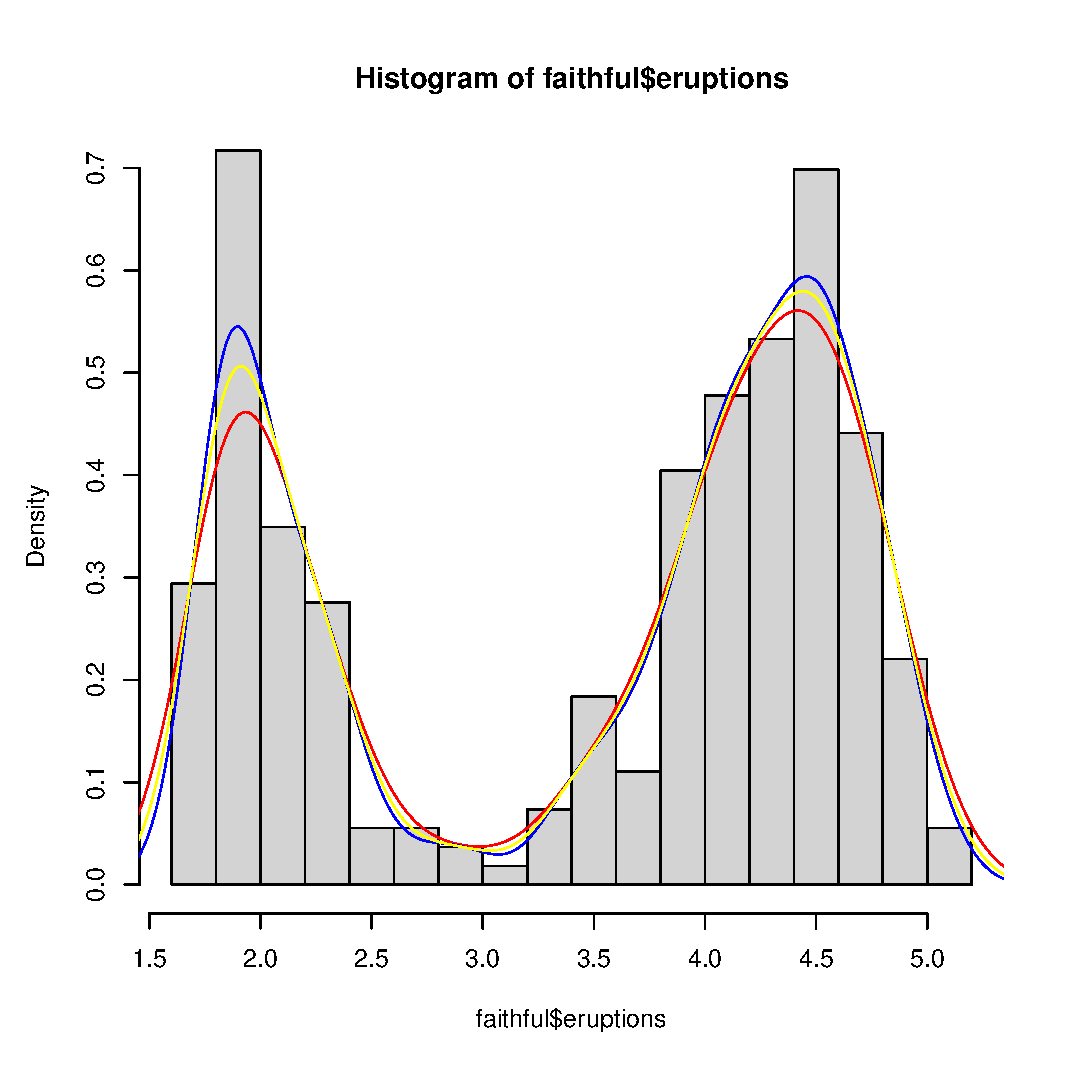
\includegraphics[width=0.9\textwidth,height=0.5\textwidth]{erpt-kernel.eps}
\end{center}
\newpage
{\LARGE\centerline{\textbf{Statistical Properties}}}
\vskip15pt
% \begin{minipage}{.9\textwidth}
    \large \noindent
    For our purpose, in the rest of this slides we assume that 
    \begin{enumerate}
        \item $K$ is a p.d.f.;
        \item $Z$ is a RV with density $K$, independent with $X$; 
        \item $K$ is symmetric, i.e. $K(x)=K(-x)$ for any $x\in\R$;\label{con-symm}
        \item $\int x^3 K(x)\mathrm{d}x=\E(Z^3)<\infty$.
    \end{enumerate}
    We found these assumptions are very common in practice, for example see Table~\ref{tabkernels}. 
    Besides, we also assume that $f''$ is continuous, and the third derivative $f^{(3)}$ of $f$ exists.
% \begin{rem}
%     From one side, Condition~\ref{con-symm} is quite reasonable for $K$ as an smoothing function. On the other hand, it is not necessary to the proofs below. Indeed, it can be replaced by a weaker condition: 
%     \begin{equation}
%         \int_{\R}xK(x)\mathrm{d}x=\E(Z)=0.
%     \end{equation}
% \end{rem}
    \begin{itemize}
        \item Bias: recalling \eqref{mean-kde}, we have 
        \begin{eqnarray}
            \bs\left\{\hat{f}(x)\right\}&=&\E\left[\hat{f}(x)\right]-f(x)\nonumber\\
            &=&(K_h*f)(x)-f(x)\nonumber\\
            &=&\int_{\R}f(x-y)K_h(y)\mathrm{d}y-f(x)\nonumber\\
            &=&\int_{\R}[f(x-y)-f(x)]K_h(y)\mathrm{d}y\nonumber\\
            &=&\int_{\R}\left[(-y)f'(x)+\frac12y^2f''(x)-\frac16y^3f^{(3)}(u^*)\right]K_h(y)\mathrm{d}y\label{taylor-1}\\
            &=&-\E(hZ)f'(x)+\frac12\E[(hZ)^2]f''(x)+o(h^2)\nonumber\\
            &=&\frac{h^2}2\var(Z)f''(x)+o(h^2).\label{bs-est1}
        \end{eqnarray}
        \item Variance:
        \begin{eqnarray}
            \var\left(\hat{f}(x)\right)&=&\frac1n\var\left(K_h(x-X_1)\right)\nonumber\\
            &=&\frac1n\E\left\{[K_h(x-X_1)-(K_h*f)(x)]^2\right\}\nonumber\\
            &=&\frac1n\left\{\E\left[K_h(x-X_1)^2\right]-(K_h*f)(x)^2\right\}.
        \end{eqnarray}
        From \eqref{bs-est1}, we have 
        \begin{equation}\label{boun1}
            (K_h*f)(x)^2=\left[f(x)+O(h^2)\right]^2=f(x)^2+O(h^2).
        \end{equation}
        Furthermore, because $K$ is symmetric, we have 
        \begin{eqnarray}
            \E\left[K_h(x-X_1)^2\right]&=&\int_{\R}K_h(x-y)^2f(y)\mathrm{d}y\nonumber\\
            &=&\frac1{h^2}\int_{\R}K\left(\frac{x-y}h\right)^2f(y)\mathrm{d}y\\
            &=&\frac1{h^2}\int_{\R}K\left(\frac{y-x}h\right)^2f(y)\mathrm{d}y\\
            &=&\frac1{h^2}\int_{\R}K(t)^2f(x+th)h\mathrm{d}t\nonumber\\
            &=&\frac1h\int_{\R}K(t)^2[f(x)+thf'(x)+o(h)]\mathrm{d}t\\
            &=&h^{-1}f(x)\|K\|_{L^2}^2+o(1),\label{boun2}
        \end{eqnarray}
        where $\|g\|_{L^2}^2:=\int_{\R}g(u)\mathrm{d}u$. 
        Combining \eqref{boun1} and \eqref{boun2}, we have 
        \begin{equation}
            \var\left(\hat{f}(x)\right)=\frac1{nh}f(x)\|K\|_{L^2}^2+O(n^{-1}).
        \end{equation}

    \item Mean Square Error (MSE) and asymptotics 
\begin{eqnarray}
    {\rm MSE}\left(\hat{f}(x)\right)&=&\bs\left\{\hat{f}(x)\right\}^2+\var\left(\hat{f}(x)\right)\nonumber\\
    &=&\left[\frac{h^2}2\var(Z)f''(x)+o(h^2)\right]^2+\frac1{nh}f(x)\|K\|_{L^2}^2+O(n^{-1})\nonumber\\
    &=&\frac{h^4}4\var(Z)^2f''(x)^2+\frac1{nh}f(x)\|K\|_{L^2}^2+o(h^2)+O(n^{-1})\\
    &\asymp&\frac{h^4}4\var(Z)^2f''(x)^2+\frac1{nh}f(x)\|K\|_{L^2}^2=:{\rm AMSE}\left(\hat{f}(x)\right)\label{amse-1}
\end{eqnarray}
where {\rm AMSE} stands for the asymptotic mean square error. 
\item Optimal local bandwidth (w.r.t. AMSE)

By differentiate \eqref{amse-1} w.r.t. $h$, we obtain 
\begin{equation}
    h^*_x=\left[\frac{f(x)\|K\|_{L^2}^2}{\var(Z)^2f''(x)^2}\right]^{1/5}n^{-1/5},
\end{equation}
and 
\begin{eqnarray}
    {\rm AMSE}^*\left(\hat{f}(x)\right)&=&\frac54\left[f(x)\|K\|_{L^2}^2\right]^{4/5}\left[\var(Z)^2f''(x)^2\right]^{1/5}n^{-4/5}\\
    &=&\frac54\left[f(x)^2f''(x)\right]^{2/5}\left[\|K\|_{L^2}^2\sqrt{\var(Z)}\right]^{4/5}n^{-4/5}.
\end{eqnarray}
Note $h^*_x$ optimizes AMSE locally, i.e. for any fixed $x\in\R$. 
\item AMISE and global optimal bandwidth 

A global measure of precision is the asymptotic mean integrated squared error (AMISE): from \eqref{amse-1} we get 
\begin{eqnarray}
    {\rm AMISE}\left(\hat{f}\right)&:=&\int_{\R}{\rm AMSE}\left(\hat{f}(x)\right)\mathrm{d}x\\
    &=&\frac{h^4}4\var(Z)^2\|f''\|_{L^2}^2+\frac1{nh}\|K\|_{L^2}^2,
\end{eqnarray}
and 
\begin{eqnarray}
    h^*&=&\left[\frac{\|K\|_{L^2}^2}{\var(Z)^2\|f''\|_{L^2}^2}\right]^{1/5}n^{-1/5},\\
    {\rm AMISE}^*\left(\hat{f}\right)&=&\frac54\left[\|K\|^2_{L^2}\sqrt{\var(Z)}\right]^{4/5}\|f''\|_{L^2}^{2/5}n^{-4/5}. \label{optamise2}
\end{eqnarray}
Comparing \eqref{optamise2} with AMISE for histogram, c.f. \eqref{L2-optamise1} in Lecture~2, the convergence rate $O(n^{-4/5})$ of kernel method is much faster than convergence rate $O(n^{-2/3})$  of histogram method. The kernel estimators are superior in rate to histograms. 

\item R code
\begin{Sinput}
set.seed(1)
x = rnorm(10000)
u = seq(-4, 4, 0.001)
plot(u, dnorm(u), col="red", type="l")
A = density(x, bw=0.1)
lines(A$x, A$y, col="black")
B = density(x, bw=0.5)
lines(B$x, B$y, col="blue")
C = density(x, bw=0.8)
lines(C$x, C$y, col="pink")
\end{Sinput}
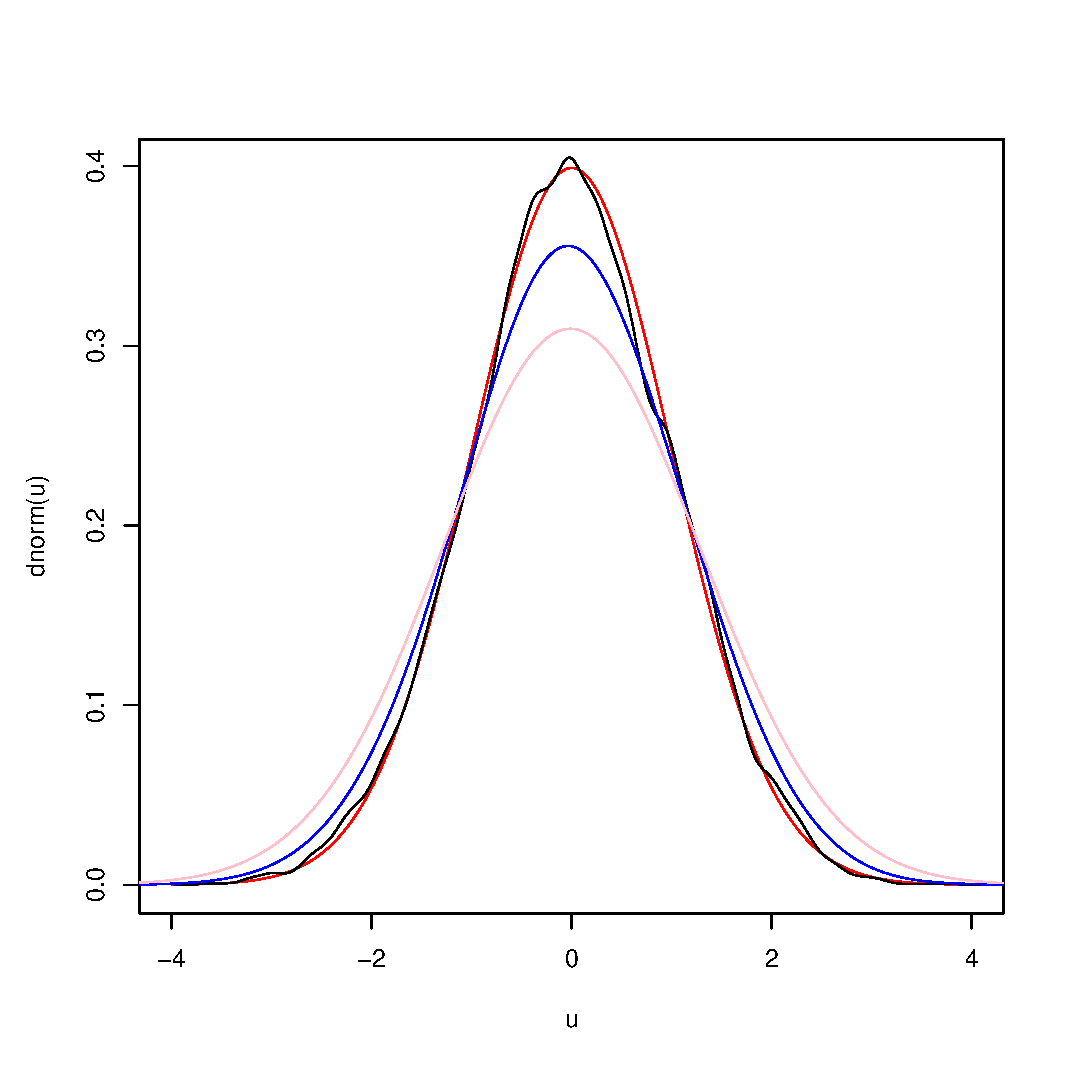
\includegraphics[width=0.9\textwidth,height=0.5\textwidth]{bias_kernel.eps}
\end{itemize}


\newpage
{\LARGE\centerline{\textbf{Refine the convergence rates}}}
\vskip15pt
% \begin{minipage}{.9\textwidth}
    \large 
    \noindent
    Nevertheless, the rate $O(n^{-4/5})$ for the MISE is not impressive if we compare it to the rate $O(n^{-1})$ that could be achieved if we knew a priori that $f$ belonged to some parametric family of densities. 

    Suppose that $f$ is $m>2$ times continuously differentiable and $f^{(m+1)}$ exists. The kernel $K$ satisfies 
    \begin{enumerate}
    \item $\int_{\R}K(u)\mathrm{d}u=1$;
    \item $\int_{\R}u^{\nu} K(u)\mathrm{d}u=0$, for all $\nu=1,\dots,m-1$;
    \item $\int_{\R}|u|^mK(u)\mathrm{d}u<\infty$,
    \item $\int_{\R}K(u)^2\mathrm{d}u<\infty$.
    \end{enumerate}
Note in this case, $K$ cannot be a p.d.f., which means the probability interpretation does not work anymore. 
\newpage
With these assumptions, we may refine the Taylor expansions in \eqref{taylor-1}, 
\begin{eqnarray*}
    &&f(x-y)-f(x)\\
    &=&(-y)f'(x)+\frac12y^2f''(x)+\cdots+\frac1{m!}(-1)^my^mf^{(m)}(x)+\frac1{(m+1)!}(-y)^{m+1}f^{(m+1)}(u^*).
\end{eqnarray*} 
Hence, 
\begin{eqnarray}
    \bs\left\{\hat{f}(x)\right\}=(-1)^m\frac{h^m}{m!}f^{(m)}(x)\int_{\R}u^mK(u)\mathrm{d}u+o(h^m).
\end{eqnarray}
\vskip 10pt
Thus, the squared bias is of the order $O(h^{2m})$ and leads to a mean square error of the order $O(n^{-2m/(2m+1)})$, which approaches the ``parametric rate'' $O(n^{-1})$ as $m\to\infty$. 
\vskip 10pt
In particular, the convergence rate $O(n^{-2m/(2m+1)})$ cannot be improved. For more detailed analysis, we refer
    \cite[Chapter~24]{Vaart98}.
% \end{minipage}

\newpage
{\LARGE\centerline{\textbf{Refine the coefficient}}}
\vskip15pt
% \begin{minipage}{.9\textwidth}
    \large 
    \noindent
    Recall \eqref{optamise2}, if we insist on the condition that $K$ is a p.d.f., the coefficient $\left[\|K\|^2_{L^2}\sqrt{\var(Z)}\right]^{4/5}$ related to kernel $K$ is invariant under linear transformation to $K$. In other words, the coefficient remains the same for replacing density $K$ of RV $Z$ with density $K'$ of any linear transformation $aZ+b$, for any $a\ne0, b\in\R$ of $Z$. Or more formally, we can write it as follows. 
\begin{prop} 
    Let $Z$ be a RV with density function $f_Z$ and $\var(Z)<\infty$. Given $a\ne0$ and $b\in \R$, denote $f_Y$ the probability density function of the RV $Y:= aZ+b$. Then 
    \begin{equation}
\|f_Z\|^2_{L^2}\sqrt{\var(Z)}=\|f_Y\|^2_{L^2}\sqrt{\var(Y)}.
    \end{equation}
\end{prop}
\begin{proof} Without loss of generality, we assume $a>0$.
    \begin{eqnarray*}
        \|f_Y\|^2_{L^2}\sqrt{\var(Y)}&=&\int_{\R}f_Y(y)^2\mathrm{d}y\sqrt{\var(aZ+b)}\\
        &=&\int_{\R}\left[\frac1af_Z\left(\frac{y-b}a\right)\right]^2\mathrm{d}y \times a\sqrt{\var(Z)}\\
        &=&\int_{\R}f_Z(z)^2\mathrm{d}z\times \sqrt{\var(Z)}\\
        &=&\|f_Z\|^2_{L^2}\sqrt{\var(Z)}
    \end{eqnarray*}
\end{proof}
Note, we don't assume $Z$ be a symmetric or mean-zero RV in the proposition above. 
\newpage
As in \cite{marron88}, kernels obtained through rescaling $K(\cdot)\mapsto \delta^{-1}K(\cdot/\delta)$, for any $\delta>0$ are said to be equivalent\footnote{equivalence relation: reflexivity, symmetry and transitivity.} to $K$. The quantity $\left[\|K\|^2_{L^2}\sqrt{\var(Z)}\right]^{4/5}$ is unified for the equivalent class. We denote it as 
\begin{equation}
    T(K):=\|K\|^{8/5}_{L^2}\left(\int_{\R}x^2K(x)\mathrm{d}x\right)^{2/5}=\left[\|K\|^2_{L^2}\sqrt{\var(Z)}\right]^{4/5},
\end{equation}
with $K$ a symmetric p.d.f. and $Z$ stands for a RV with density $K$.

We can rewrite \eqref{optamise2} as 
\begin{equation}\label{optamise3}
    {\rm AMISE}^*\left(\hat{f}\right)=\frac54T(K)\|f''\|_{L^2}^{2/5}n^{-4/5}.
\end{equation}
A question of immediate interest is to find the kernel that minimizes $T(K)$. 
\cite{epanechnikov} shows 
\begin{equation}
    K_e(t)=\frac3{4\sqrt{5}}(1-t^2/5)\bone_{\{|t|\le \sqrt{5}\}}
\end{equation}
minimizes the function $T(K)$.

\newpage 
\begin{table}[ht]
    \centering
    \caption{Efficiency Constants for Different Kernels}
    \begin{tabular}{lcc}
    \toprule
    Kernel       & $T(K)$\\
    \midrule
    Uniform      & 0.3701072 \\
    Triangle     & 0.3530746 \\
    Epanechnikov & 0.3490865 \\
    Quartic      & 0.3507990 \\
    Triweight    & 0.3528512 \\
    Cosine       & 0.3492399 \\
    Gaussian     & 0.3633424 \\
    \bottomrule
    \end{tabular}
    \label{tab:efficiency_constants}
    \end{table}

\begin{Schunk}
\begin{Sinput}
    # Load necessary library
    library(stats)
    
    # Define the kernels
    kernels <- list(
      uniform = function(x) ifelse(abs(x) <= 1, 0.5, 0),
      epanechnikov = function(x) ifelse(abs(x) <= 1, 3/4 * (1 - x^2), 0),
      quartic = function(x) ifelse(abs(x) <= 1, 15/16 * (1 - x^2)^2, 0),
      triweight = function(x) ifelse(abs(x) <= 1, 35/32 * (1 - x^2)^3, 0),
      cosine = function(x) ifelse(abs(x) <= 1, pi/4 * cos(pi/2 * x), 0),
      gaussian = function(x) dnorm(x),
      triangle = function(x) ifelse(abs(x) <= 1, 1 - abs(x), 0)
    )
    
    # Function to compute the L2 norm
    L2_norm <- function(K, lower = -Inf, upper = Inf) {
      sqrt(integrate(function(x) K(x)^2, lower, upper)$value)
    }
    #Function to compute the second moment
    second_moment <- function(K, lower = -Inf, upper = Inf) {
      integrate(function(x) x^2 * K(x), lower, upper)$value
    }
    
    # Function to compute the efficiency constant
    efficiency_constant <- function(K) {
      L2 <- L2_norm(K)
      second_mom <- second_moment(K)
      L2^(8/5) * second_mom^(2/5)
    }
    
    # Compute the efficiency constants for each kernel
    efficiency_constants <- sapply(kernels, efficiency_constant)
    
    # Print the results
    print(efficiency_constants)
    
\end{Sinput}
\end{Schunk}
\newpage
{\LARGE\centerline{\textbf{Summary}}}
\vskip25pt
\begin{minipage}{.9\textwidth}
    \Large 
    \begin{itemize}
    \item The convergence rate $O(n^{-4/5})$ (or $O(n^{-2m/(2m+1)})$) of kernel method is better than that of histogram method.
    \item Even through $T(K)$ is not the same for different kernels, it does not matter for the asymptotic behaviour of AMISE. 
    \item The roughness of kernel matters, but not much. See the table~\ref{tab:efficiency_constants}.    
    \end{itemize}
    \vskip 10pt
    {\huge Using chatGPT to code \& visualize it!}
\end{minipage}

\newpage
\bibliographystyle{apalike}
\bibliography{ref}
% \begin{thebibliography}{}

%     \bibitem[Boyd and Steele, 1978]{boydsteele78}
%     Boyd, D.~W. and Steele, J.~M. (1978).
%     \newblock Lower bounds for nonparametric density estimation rates.
%     \newblock {\em Ann. Statist.}, 6(4):932--934.
    
%     \bibitem[Doane, 1976]{doane76}
%     Doane, D.~P. (1976).
%     \newblock Aesthetic frequency classifications.
%     \newblock {\em Amer. Statist.}, 30(4):181--183.
    
%     \bibitem[Dudley, 2002]{Dudley02}
%     Dudley, R.~M. (2002).
%     \newblock {\em Real Analysis and Probability}.
%     \newblock Cambridge Studies in Advanced Mathematics. Cambridge University Press, Cambridge, 2 edition.
    
%     \bibitem[Freedman and Diaconis, 1981]{FreedmanDiaconis81}
%     Freedman, D. and Diaconis, P. (1981).
%     \newblock On the histogram as a density estimator: $L_2$ theory.
%     \newblock {\em Probab. Theory Related Fields}, 57(4):453--476.
    
%     \bibitem[Garthwaite et~al., 2002]{garthwaite02}
%     Garthwaite, P.~H., Jolliffe, I.~T., and Jones, B. (2002).
%     \newblock {\em Statistical inference}.
%     \newblock OUP Oxford.
    
%     \bibitem[Scott, 1979]{scott79}
%     Scott, D.~W. (1979).
%     \newblock {On optimal and data-based histograms}.
%     \newblock {\em Biometrika}, 66(3):605--610.
    
%     \bibitem[Scott, 2015]{scott15}
%     Scott, D.~W. (2015).
%     \newblock {\em Multivariate density estimation: theory, practice, and visualization}.
%     \newblock Wiley Series in Probability and Statistics. John Wiley \& Sons, 2nd edition.
    
%     \bibitem[Sturges, 1926]{sturges26}
%     Sturges, H.~A. (1926).
%     \newblock The choice of a class interval.
%     \newblock {\em J. Amer. Statist. Assoc.}, 21(153):65--66.
    
%     \end{thebibliography}
    
\end{document}